\section{FFT (Inverse) Fast Fourier Transform Function}

\subsection{Usage}

Computes the Discrete Fourier Transform (DFT) of a vector using the
Fast Fourier Transform technique.  The general syntax for its use is
\begin{verbatim}
  y = fft(x,n,d)
\end{verbatim}
where \verb|x| is an \verb|n|-dimensional array of numerical type.
Integer types are promoted to the \verb|double| type prior to 
calculation of the DFT. The argument \verb|n| is the length of the
FFT, and \verb|d| is the dimension along which to take the DFT.  If
|n| is larger than the length of \verb|x| along dimension \verb|d|,
then \verb|x| is zero-padded (by appending zeros) prior to calculation
of the DFT.  If \verb|n| is smaller than the length of \verb|x|  along
the given dimension, then \verb|x| is truncated (by removing elements
at the end) to length \verb|n|.  

If \verb|d| is omitted, then the DFT is taken along the first 
non-singleton dimension of \verb|x|.  If \verb|n| is omitted, then
the DFT length is chosen to match of the length of \verb|x| along
dimension \verb|d|.  

Note that FFT support on Linux builds requires availability
of the FFTW libraries at compile time.  On Windows and Mac OS
X, single and double precision FFTs are available by default.
\subsection{Function Internals}

The output is computed via
\[
y(m_1,\ldots,m_{d-1},l,m_{d+1},\ldots,m_{p}) = 
\sum_{k=1}^{n} x(m_1,\ldots,m_{d-1},k,m_{d+1},\ldots,m_{p})
e^{-\frac{2\pi(k-1)l}{n}}.
\]

For the inverse DFT, the calculation is similar, and the arguments
have the same meanings as the DFT:
\[
y(m_1,\ldots,m_{d-1},l,m_{d+1},\ldots,m_{p}) = 
\frac{1}{n} \sum_{k=1}^{n} x(m_1,\ldots,m_{d-1},k,m_{d+1},\ldots,m_{p})
e^{\frac{2\pi(k-1)l}{n}}.
\]
The FFT is computed using the FFTPack library, available from 
netlib at \verb|http://www.netlib.org|.  Generally speaking, the 
computational cost for a FFT is (in worst case) \verb|O(n^2)|.
However, if \verb|n| is composite, and can be factored as
\[
n = \prod_{k=1}^{p} m_k,
\]
then the DFT can be computed in 
\[
O(n \sum_{k=1}^{p} m_k)
\]
operations.  If \verb|n| is a power of 2, then the FFT can be
calculated in \verb|O(n log_2 n)|.  The calculations for the
inverse FFT are identical.
\subsection{Example}

The following piece of code plots the FFT for a sinusoidal signal:
\begin{verbatim}
--> t = linspace(0,2*pi,128);
--> x = cos(15*t);
--> y = fft(x);
--> plot(t,abs(y));
\end{verbatim}
The resulting plot is:


\centerline{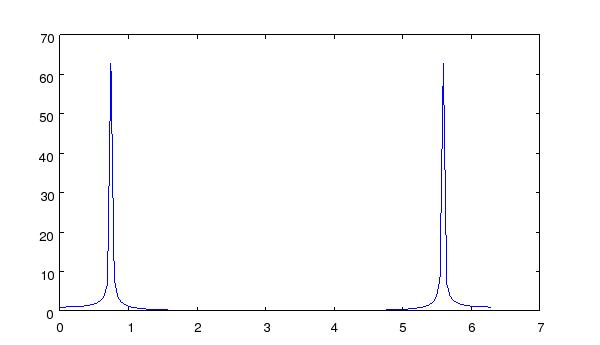
\includegraphics[width=8cm]{fft1}}


The FFT can also be taken along different dimensions, and with padding 
and/or truncation.  The following example demonstrates the Fourier
Transform being computed along each column, and then along each row.
\begin{verbatim}
--> A = [2,5;3,6]

A = 
 2 5 
 3 6 

--> real(fft(A,[],1))

ans = 
  5 11 
 -1 -1 

--> real(fft(A,[],2))

ans = 
  7 -3 
  9 -3 
\end{verbatim}
Fourier transforms can also be padded using the \verb|n| argument.  This
pads the signal with zeros prior to taking the Fourier transform.  Zero
padding in the time domain results in frequency interpolation.  The
following example demonstrates the FFT of a pulse (consisting of 10 ones)
with (red line) and without (green circles) padding.
\begin{verbatim}
--> delta(1:10) = 1;
--> plot((0:255)/256*pi*2,real(fft(delta,256)),'r-');
--> hold on
--> plot((0:9)/10*pi*2,real(fft(delta)),'go');
\end{verbatim}
The resulting plot is:


\centerline{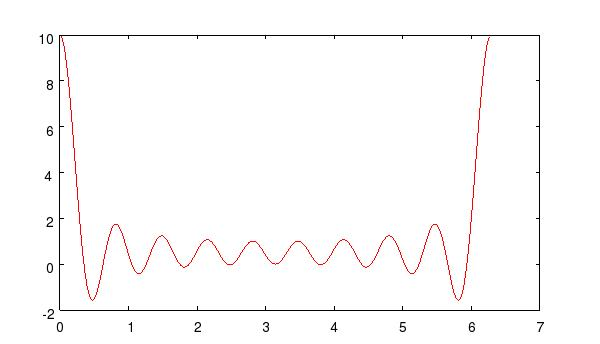
\includegraphics[width=8cm]{fft2}}

